\documentclass[handout]{beamer}
\usepackage{multicol}
\usepackage{xy}
\everymath{\displaystyle}
\mode<presentation>
{\usetheme{Warsaw}\setbeamercovered{dynamic}}
\usecolortheme{crane}
\usepackage{beamerfoils}
\pgfdeclareimage[height=1in]{university-logo}{ISULogo}
\logo{\pgfuseimage{university-logo}}
\setbeamertemplate{navigation symbols}{}
\title[\S10]{Section 10\\Combinatorics applications}
\author{Dr Marcus Bishop}
\subject{Math 104}
\beamerdefaultoverlayspecification{<+->}
\theoremstyle{definition}
\newtheorem{remark}{Remark}
\newtheorem{impact}{Impact}
\newtheorem{situation}{Situation}
\newtheorem{question}{Question}
\usepackage{arev}
\usepackage{tensor}
\newcommand\npr[2]{\tensor[_{#1}]P{_{#2}}}
\newcommand\ncr[2]{\tensor[_{#1}]C{_{#2}}}
\usepackage{cancel}
\newcommand{\hs}{\alert{\varheart}}
\newcommand{\ds}{\alert{\vardiamond}}
\newcommand{\s}{\spadesuit}
\newcommand{\cs}{\clubsuit}
\begin{document}
\begin{frame}\titlepage\end{frame}
\LogoOff

\begin{frame}{Poker outline}
\begin{itemize}
\item Dealer deals five cards from standard deck
to each player
\item Selection of five cards called a \alert{hand}
\item For simplicity, we imagine all five cards in player's hand
\item In reality, some cards lying face up on table
\item Players make bets and/or replace cards
\item Finally, player with \alert{best hand} wins
\item Nine categories of poker hands:
\begin{tabular}{lll}
Straight flush&Four-of-a-kind&Full house\\
Flush&Straight&Three-of-a-kind\\
Two pairs&One pair&High card
\end{tabular}
\item Strength of hand determined by probability
%(although listed from best to worst above)
\item The smaller the probability, the stronger the hand
\item If two players have same type of hand, tie
broken in manner depending on type of hand
\end{itemize}
\end{frame}

\begin{frame}{Playing cards}
\begin{itemize}
\item Recall that deck has cards of thirteen \alert{ranks},
$A,K,Q,J,10,9,8,7,6,5,4,3,2$
listed from highest to lowest
\item Each rank has four cards, one of each \alert{suit} $\hs,\ds,\cs,\s$
\item Thus deck has $13\cdot 4=52$ cards
\end{itemize}
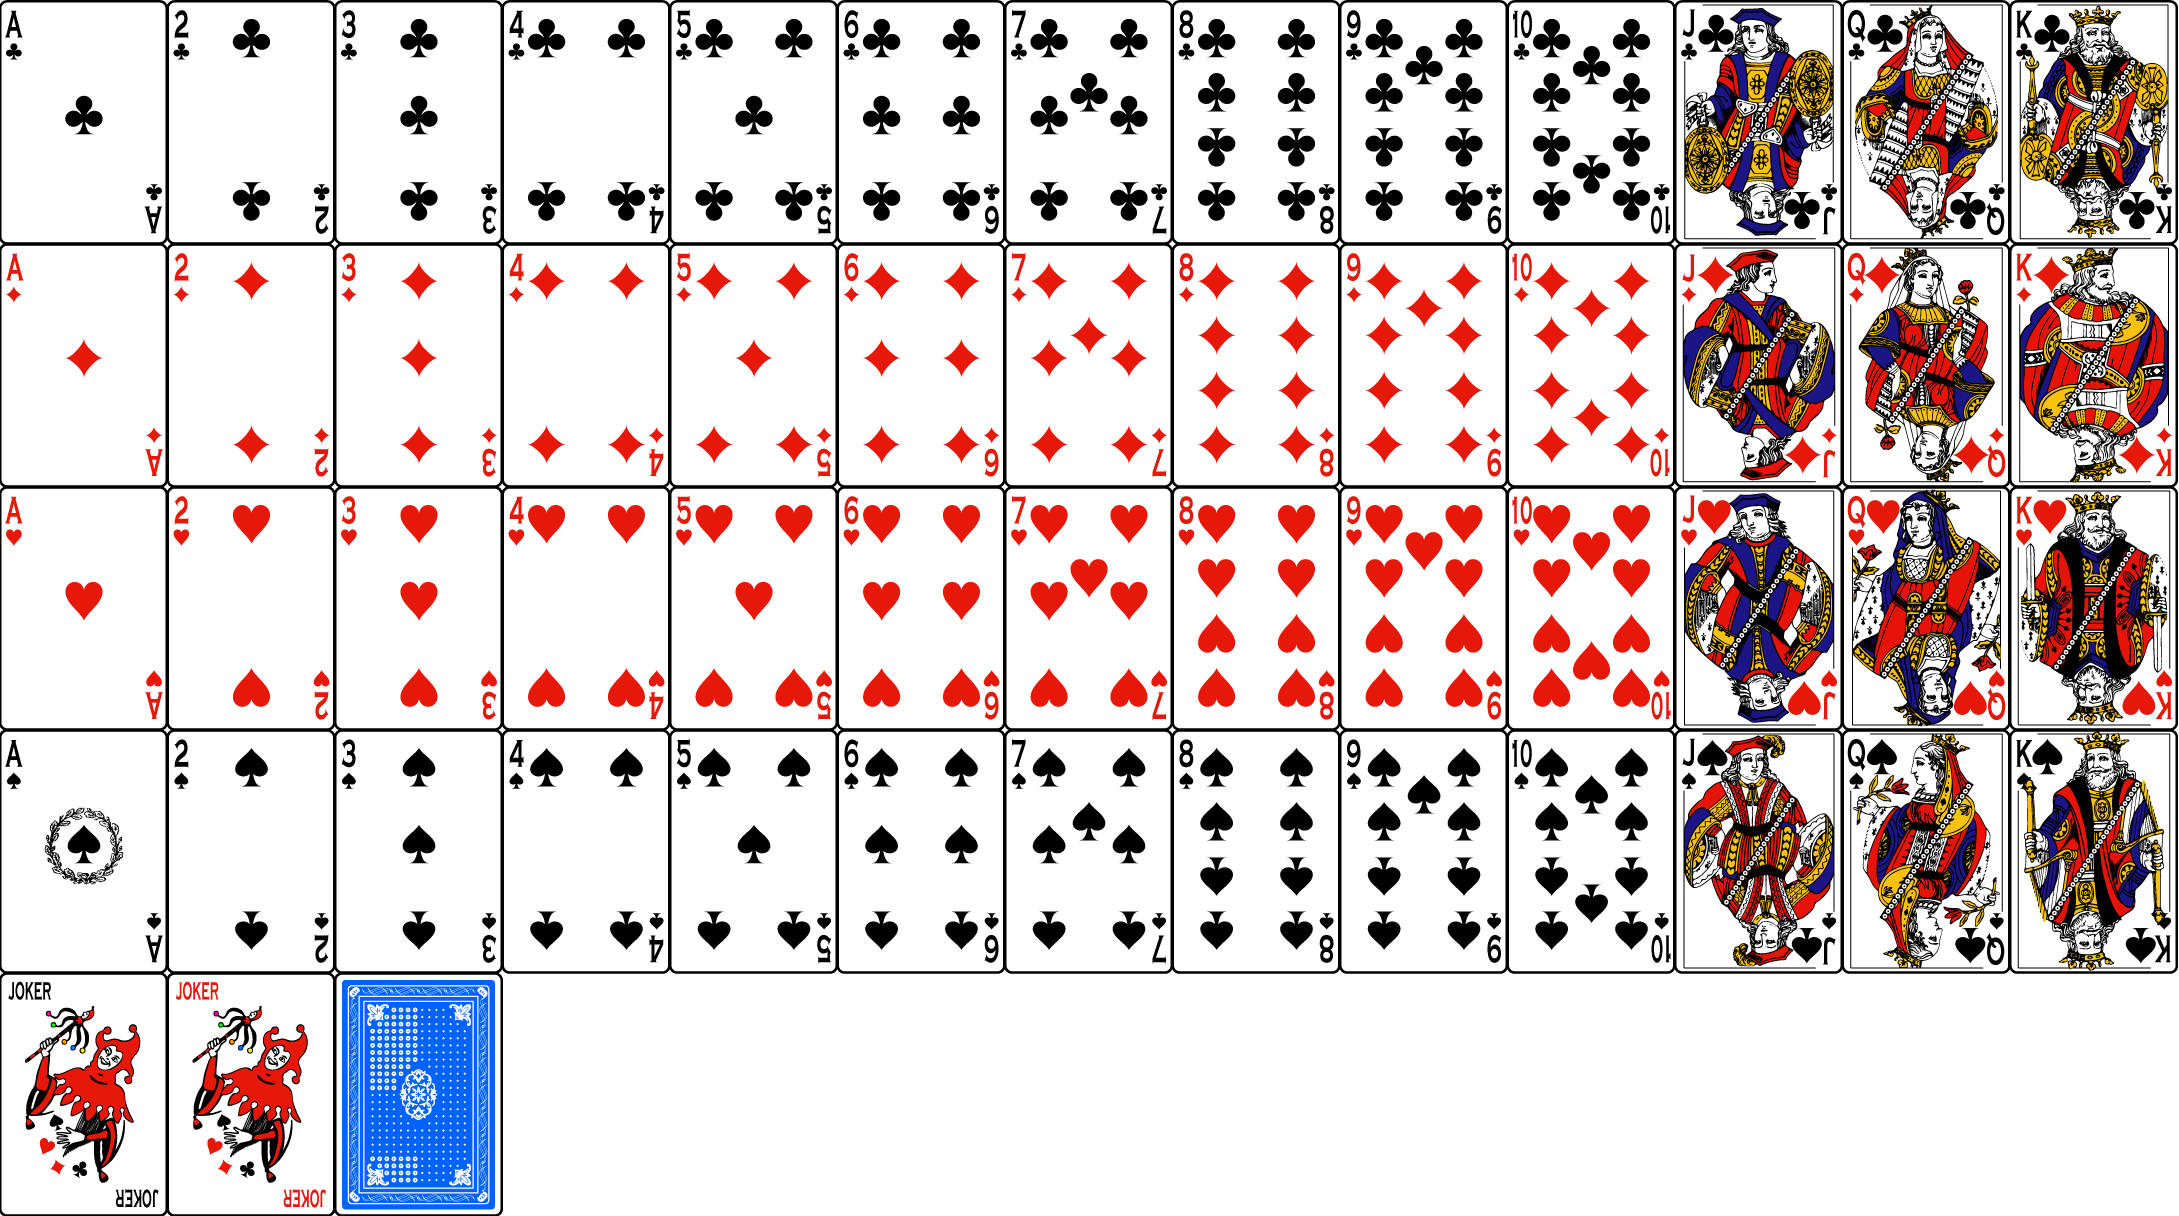
\includegraphics[scale=.3]{cards}
\end{frame}

\begin{frame}{Poker basics}
\begin{itemize}
\item So $\ncr{52}{5}=2,598,960$ the number of possible hands
\item Will first calculate probability that player dealt
hand of particular type
\item This probability not altered by fact that other cards
might have already been dealt to other players
\item \dots provided that those cards \alert{not exposed to player}
\item However, some variants of poker involve exposing cards
\end{itemize}
\begin{example}
If card of suit $\hs$ lying face up on table, affects probability
that next card drawn will have suit $\hs$
\end{example}
\end{frame}

\begin{frame}{Four of a kind}
\begin{itemize}
\item Hand called \alert{four-of-a-kind} if four cards have
same rank
\item Fifth card and common rank of first four cards unimportant
\item However, if another player also has four-of-a-kind,
then player with four cards of highest rank wins
\begin{example} $8\hs,8\ds,8\cs,8\s,10\cs$ a four-of-a-kind\end{example}
\begin{example} $9\hs,9\ds,9\cs,9\s,3\hs$ a four-of-a-kind,
and beats hand above\end{example}
\end{itemize}
\end{frame}

\begin{frame}{Counting four-of-a-kinds }
\begin{itemize}
\item How many ways to form four-of-a-kind?
\item Thirteen ways to choose common rank of four cards
\item $48$ cards have rank different from common rank
\item So $48$ ways to choose fifth card
\item Thus $13\cdot 48=624$ possible four-of-a-kinds
\item So $\frac{624}{2598960}=\frac{1}{4165}\approx 0.00024$
the probability of being dealt four-of-a-kind
\end{itemize}
\end{frame}

\begin{frame}{Full house}
\begin{itemize}
\item Hand called a \alert{full house} if three
cards have same rank and remaining two have same rank
\begin{example} $8\hs,8\ds,8\cs,10\s,10\ds$ a full house\end{example}
\item If another player has full house, then player with
three cards of highest rank wins
\begin{example} $9\hs,9\ds,9\cs,7\hs,7\s$ a full house,
and beats hand above\end{example}
\end{itemize}
\end{frame}

\begin{frame}{Counting full houses}
\begin{itemize}
\item First choose two common ranks
\item $13$~ways to choose first rank
\item $12$~ways to choose second rank
\item Next, choose three cards of first rank
\item $\ncr{4}{3}=4$ ways
\item Finally, choose two cards of second rank
\item $\ncr{4}{2}=6$ ways
\item So $13\cdot 12\cdot 4\cdot 6=3744$ possible full houses
\item So $\frac{3744}{2598960}=\frac{6}{4165}\approx 0.01444$
the probability of begin dealt a full house
\item Note that $\frac{6}{4165}>\frac{1}{4165}$,
so four-of-a-kind beats full house
\end{itemize}
\end{frame}

\begin{frame}{Three-of-a-kind}
\begin{itemize}
\item Hand called \alert{three-of-a-kind} if
three cards have same rank
\item Remaining two cards should have rank different
from first three (else hand is four-of-a-kind)
\item Also, remaining cards should have rank
different from one another (else hand is full house)
\begin{example} $8\hs,8\ds,8\cs,Q\hs,10\cs$ a three-of-a-kind\end{example}
\end{itemize}
\end{frame}

\begin{frame}{Counting three-of-a-kinds}
\begin{itemize}
\item $13$ choices for common rank of three cards
\item $\ncr{4}{3}=4$ choices for three cards of rank chosen above
\item $52-4=48$ cards have rank different from rank chosen above
\item So $48$~choices for fourth card
\item $48-4=44$~cards have rank different from two ranks chosen above
\item So $44$~choices for fifth card
\item However, order in which fourth and fifth cards selected unimportant
\item $48\cdot 44$ counts each choice \alert{twice}
\item Hence divide final answer by $2$
\item So $\frac{13\cdot 4\cdot 48\cdot 44}{2}=54,912$ three-of-a-kinds
\end{itemize}
\end{frame}

\begin{frame}{Another way to count three-of-a-kinds}
\begin{itemize}
\item $13$ choices for common rank of three cards
\item $\ncr{4}{3}=4$ choices for three cards of rank chosen above
\item $\ncr{12}{2}=66$ choices for ranks of two remaining cards
\item $4$~choices for suit of fourth card 
\item $4$~choices for suit of fifth card 
\item So $13\cdot 4\cdot 66\cdot 4\cdot 4=54,912$ three-of-a-kinds
\item Agrees with previous calculation
\item So $\frac{54912}{2598960}=\frac{88}{4165}\approx 0.02113$ the probability
of being dealt four-of-a-kind
\end{itemize}
\end{frame}

\begin{frame}
\begin{situation}
\begin{itemize}
\item You have $3\hs,8\hs,J\hs,Q\hs,5\s$
\item Would like to replace $5\s$ with card of suit $\hs$ to complete flush
\item You know your opponent has two pairs (by telepathy or otherwise)
\item She would like to exchange fifth card to complete full house
\end{itemize}
\end{situation}
\begin{itemize}
\item $52-5=47$ cards remain unknown to you
\item You have four $\hs$'s so nine $\hs$'s remain
\item So you receive $\hs$ with probability $\frac{9}{47}$
\item But $\frac{9}{47}$ \alert{not} your probability of winning!
\item Opponent must also \alert{fail} to complete her full house,
since full house beats flush
\end{itemize}
\end{frame}

\begin{frame}
\begin{itemize}
\item Opponent has two pairs
\item For concreteness, suppose she has $4\s,4\cs,5\ds,5\s$
\item So she completes full house if she receives $4$ or $5$
\item So she \alert{fails} to complete full house
if rank of card dealt not $4$ \alert{and} not $5$
\item Since she has two $4$'s, two remain unknown to her
\item Since has two $5$'s, two remain unknown to her
\item So $47-4=43$ unknown cards are not $4$ and not $5$
\item Thus $\frac{43}{47}$ her probability of failing
\item So $\frac{9}{47}\cdot\frac{43}{47}\approx 0.1752$
your probability of winning
\end{itemize}
\end{frame}

\begin{frame}
\begin{situation}
\begin{itemize}
\item You have $J\hs,J\cs,4\s,4\hs,Q\cs$
\item You could exchange one card, hoping to complete full house
\item You could also exchange $4\s,4\hs,Q\cs$, hoping to build better hand
\end{itemize}
\end{situation}
\begin{itemize}
\item Two of $47$ cards unknown to you are $J's$, two are $4$'s
\item Thus $\frac{4}{47}=\frac{1}{12}\approx 0.0851$ you probability
of completing full house
\end{itemize}
\end{frame}

\begin{frame}
\begin{itemize}
\item Suppose instead you exchange $4\s,4\hs,Q\cs$
\item First calculate probability that exactly one of new cards
has rank $J$
\item Then you have three-of-a-kind
\item Also, if two remaining cards have same rank,
then you have full house
\item $47$ cards remain unknown to you
\item They include two $J$'s
\item So $45$ unknown cards have rank other than $J$
\item So $\frac{45}{47}\cdot\frac{44}{46}\cdot\frac{2}{45}
+\frac{45}{47}\cdot\frac{2}{46}\cdot\frac{44}{45}
+\frac{2}{47}\cdot\frac{45}{46}\cdot\frac{44}{45}\approx 0.1221$
the probability of receiving one $J$ and two cards other than $J$
\end{itemize}
\end{frame}

\end{document}

